\documentclass[11pt,journal]{article}
%\usepackage{hyperref}
%\usepackage[breaklinks]{hyperref}
\usepackage{breakurl}
\usepackage{url}
\usepackage{listings}
\usepackage{courier}
\usepackage{amsmath}
\usepackage{graphicx}
\graphicspath{ {/home/agata/Documents/coursework/SensorNetworks/Lab2/} }
%\ifCLASSOPTIONcompsoc
% IEEE Computer Society needs nocompress option
% requires cite.sty v4.0 or later (November 2003)
\usepackage[nocompress]{cite}

%\else
% normal IEEE
\usepackage{cite}
%\fi

\hyphenation{op-tical net-works semi-conduc-tor}
\addtolength{\oddsidemargin}{-.875in}
\addtolength{\evensidemargin}{-.875in} 
\addtolength{\textwidth}{1.75in}

\addtolength{\topmargin}{-.875in}
\addtolength{\textheight}{1.75in}

\begin{document}
	\title{Sensor Networks and Mobile Data Comminucation, Assignment 2}
	
	\author{UID: 1690550}% <-this % stops a space
		%\protect\\
		%\thanks{}}
	
	% The paper headers



	% IEEEtran.cls defaults to using nonbold math in the Abstract.
	% This preserves the distinction between vectors and scalars. However,
	% if the journal you are submitting to favors bold math in the abstract,
	% then you can use LaTeX's standard command \boldmath at the very start
	% of the abstract to achieve this. Many IEEE journals frown on math
	% in the abstract anyway. In particular, the Computer Society does
	% not want either math or citations to appear in the abstract.
	
	% Note that keywords are not normally used for peerreview papers.
	
	% make the title area
	\maketitle
	
	
	% To allow for easy dual compilation without having to reenter the
	% abstract/keywords data, the \IEEEcompsoctitleabstractindextext text will
	% not be used in maketitle, but will appear (i.e., to be "transported")
	% here as \IEEEdisplaynotcompsoctitleabstractindextext when compsoc mode
	% is not selected <OR> if conference mode is selected - because compsoc
	% conference papers position the abstract like regular (non-compsoc)
	% papers do!
	%\IEEEdisplaynotcompsoctitleabstractindextext
	% \IEEEdisplaynotcompsoctitleabstractindextext has no effect when using
	% compsoc under a non-conference mode.
	
	
	% For peer review papers, you can put extra information on the cover
	% page as needed:
	% \ifCLASSOPTIONpeerreview
	% \begin{center} \bfseries EDICS Category: 3-BBND \end{center}
	% \fi
	%
	% For peerreview papers, this IEEEtran command inserts a page break and
	% creates the second title. It will be ignored for other modes.
	%\IEEEpeerreviewmaketitle

	\section{Log-distance propagation loss model\cite{log distance doc} (Methods 1)}
	The equation to calculate loss in the log-distance propagation model is:
	\[L = L_0 + 10nlog_{10}(\dfrac{d}{d_0})\] 
	with $L$ being the relative path loss, $L_0$ the path loss at reference distance $d_0$, n being the path loss distance exponent, and d the distance at which we're looking.
	
	\subsection{Initial readings}
	Before we can discuss the effects of changing the parameters, we need to take some initial readings that will be considered "normal", to which we can compare.
	
	Note that 802.11b standard lists 20 dBm as the standard transmission power for WiFi, with -100 dBm being the minimal received signal power. However, we are interested in a much more narrow range. To fine-tune it even further, just this once we take readings at the distance ranging from 180 to 180.9 m, at 0.05m intervals. The results are show in the graph below.
		\begin{figure}[h]
		\centering
		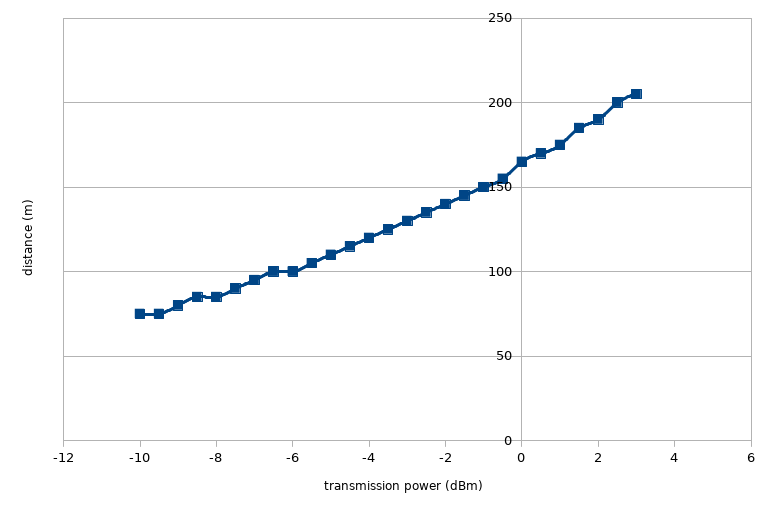
\includegraphics[scale=0.6]{graph_initial.png}
		\caption{Maximum transmission distance for the given transmission power.}
	\end{figure}
	
	These results will be considered the "normal" output, to which we can compare the outcomes of any modifications. Further readings may be taken at a different range of both power and output, when so requested.
	
	The model has 3 attributes: path loss exponent, reference distance, and reference loss. Reference distance and loss come together, and we shall look at them first. 
	
	\subsection{Reference loss and distance}
	This pair of attributes describes how much power we lose at the reference distance from the source. It is included in the model to avoid taking $log_{10}(0)$ which tends to $-\infty$. Therefore there is no point in attempting to get a reading at a shorter distance, as it will not be meaningful. 
	
	Effectively, these attributes describe how much to add to the loss, to account for skipping the reference distance in the calculations. It should not come as a surprise that increasing the reference loss, decreases transmission range. 
	
	Using the original range of values for power and distance, we vary the reference loss from 19 to 20 dB, in 0.1 dB intervals. The power is fixed at 0.1 dBm. The outcome is shown in the graph below.
	
	\begin{figure}[h]
		\centering
		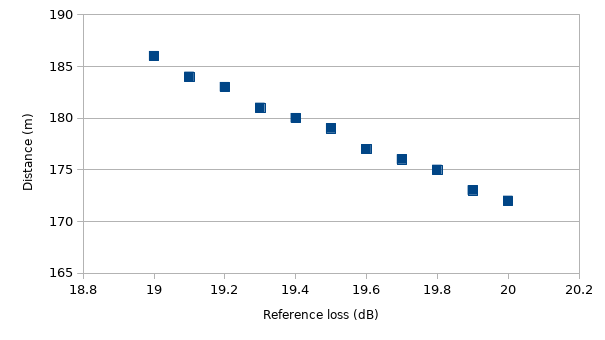
\includegraphics[scale=0.6]{graph_log_refloss.png}
		\caption{Maximum distance reached for a given reference loss.}
	\end{figure}
	
	It is not ideal to increase the reference distance, as it will limit the range at which we can take the readings. Attempting to find the loss at a distance less than the reference distance, will return the transmission power.

	\subsection{exponent}
	The other parameter in the model is the exponent $n$. Recall the model equation:
		\[L = L_0 + 10nlog_{10}(\dfrac{d}{d_0})\] 
		\[ = L_o + 10log_{10}((\dfrac{d}{d_0})^n)\]
		
	Therefore, we can expect an exponential decrease in the maximum distance reached, as we increase the exponent. Our findings, summarised in the graph in Fig. 3 indeed demonstrate this trend. (Readings taken at transmission power 0.1 dBm.)
	
	
	\begin{figure}[h]
		\centering
		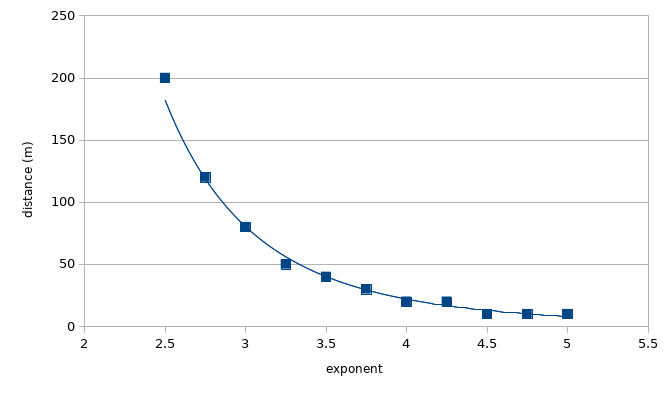
\includegraphics[scale=0.6]{graph_log_exponent.png}
		\caption{Maximum distance reached for a given exponent.}
	\end{figure}
	\pagebreak
	\section{Friis propagation loss model\cite{friis doc} (Methods 2a)}
	This model has been first introduced by H. Friis in 1946\cite{Friis note}. In its simplest form, the loss is calculated as a ratio between transmitter's power and receiver's power. The equation is:
	
	\[\frac{P_r}{P_t} = G_tG_r(\frac{\lambda}{4\pi d})^2  \]
	Where $d$ is the distance, $\lambda$ is the wavelength, $G_t$ and $G_r$ are antenna gains. They are inversely proportional to $\lambda ^2$, wavelength squared. Thus, this makes the loss proportionate to the square of wavelength. For comparison, the relation in the log distance propagation loss model is exponential.
		
	As described by Shaw\cite{Shaw}, this simple form has multiple limitations. It does not give a meaningful answer for a distance $d$ shorter than the wavelength. It requires a single value of wavelength, which implies a very narrow bandwidth. It also only works for free space with no obstacles and no refraction taking place.
	
	Therefore, the NS-3 model and other modern applications often use a more complicated version of the equation, which gives the receiver's power:
	
	\[P_r = \dfrac{P_tG_rG_t\lambda ^2}{(4\pi d)^2 L}\]
	
	The additional parameter $L$ is the system loss to correct for the idealistic assumptions.
	
	In the following simulation we will use $\lambda = 0.10$ m. The NS-3 model requires the following three attributes: minimum distance $d_0$, system loss $L$, and frequency $f$.
	
	The frequency can be calculated from the wavelength:
	
	\[ f = \dfrac{c}{\lambda} =  \dfrac{3\times 10^8}{0.1}= 3 \times 10^9 \approx 3 \text{GHz} \]
	
	We will leave the system loss as the default value of 1, and the minimum distance likewise as the default 0.5. m.
	
	The readings, taken for the same values of transmission power and distance, as in the log distance propagation loss model, are shown on the graph in Fig. 4 in blue, while the orange points show the distance reached in the log distance model simulation.
	
	Both models show a similar trend, however in the Friis model the distance reached is consistently lower at this range, although it increases at a faster rate within this range. However, if we extrapolate the functions, we can expect the log distance model to overtake Friis model, as it is an exponential function against a quadratic one.
	
	\begin{figure}[h]
		\centering
		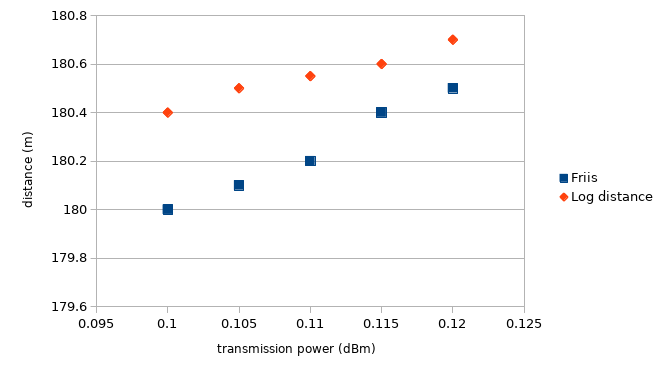
\includegraphics[scale=0.6]{graph_friis2.png}
		\caption{Maximum distance reached for a given transmission power, as simulated with the Friis model.}
	\end{figure}
	
	\section{Range propagation loss model\cite{range doc} (Methods 2b)}
	This is the simplest possible propagation loss model, and a rather abstract and unrealistic one. It depends only on the distance between the transmitter and the receiver. If the distance is greater than the maximum range, the packets are received at negligible power. Anything closer than that to the transmitter receives at the transmit power level.
	
	We set the maximum range to 180.5, and unsurprisingly for all our test transmitter power values, the packages are received up to the maximum range. Again we compare it to the log distance propagation loss model.
	
	\begin{figure}[h]
		\centering
		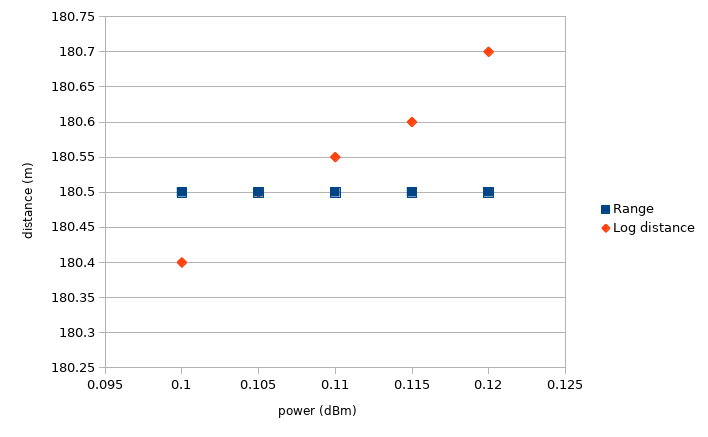
\includegraphics[scale=0.6]{graph_range.png}
		\caption{Maximum distance reached for a given transmission power, as simulated with the range model.}
	\end{figure}

	\section{Two-ray ground propagation loss model\cite{two ray doc} (Methods 2)}
	This model assumes that the signal travels from the transmitter to the receiver via two paths simultaneously: the direct line of sight and a path in which the signal is reflected off the ground, as shown in Fig. 6\footnote{source of the diagram: \url{https://commons.wikimedia.org/wiki/File:2-Ray_Ground_Reflection.png}, author: Wikipedia user Derekjc}.
	
	\begin{figure}[h]
		\centering
		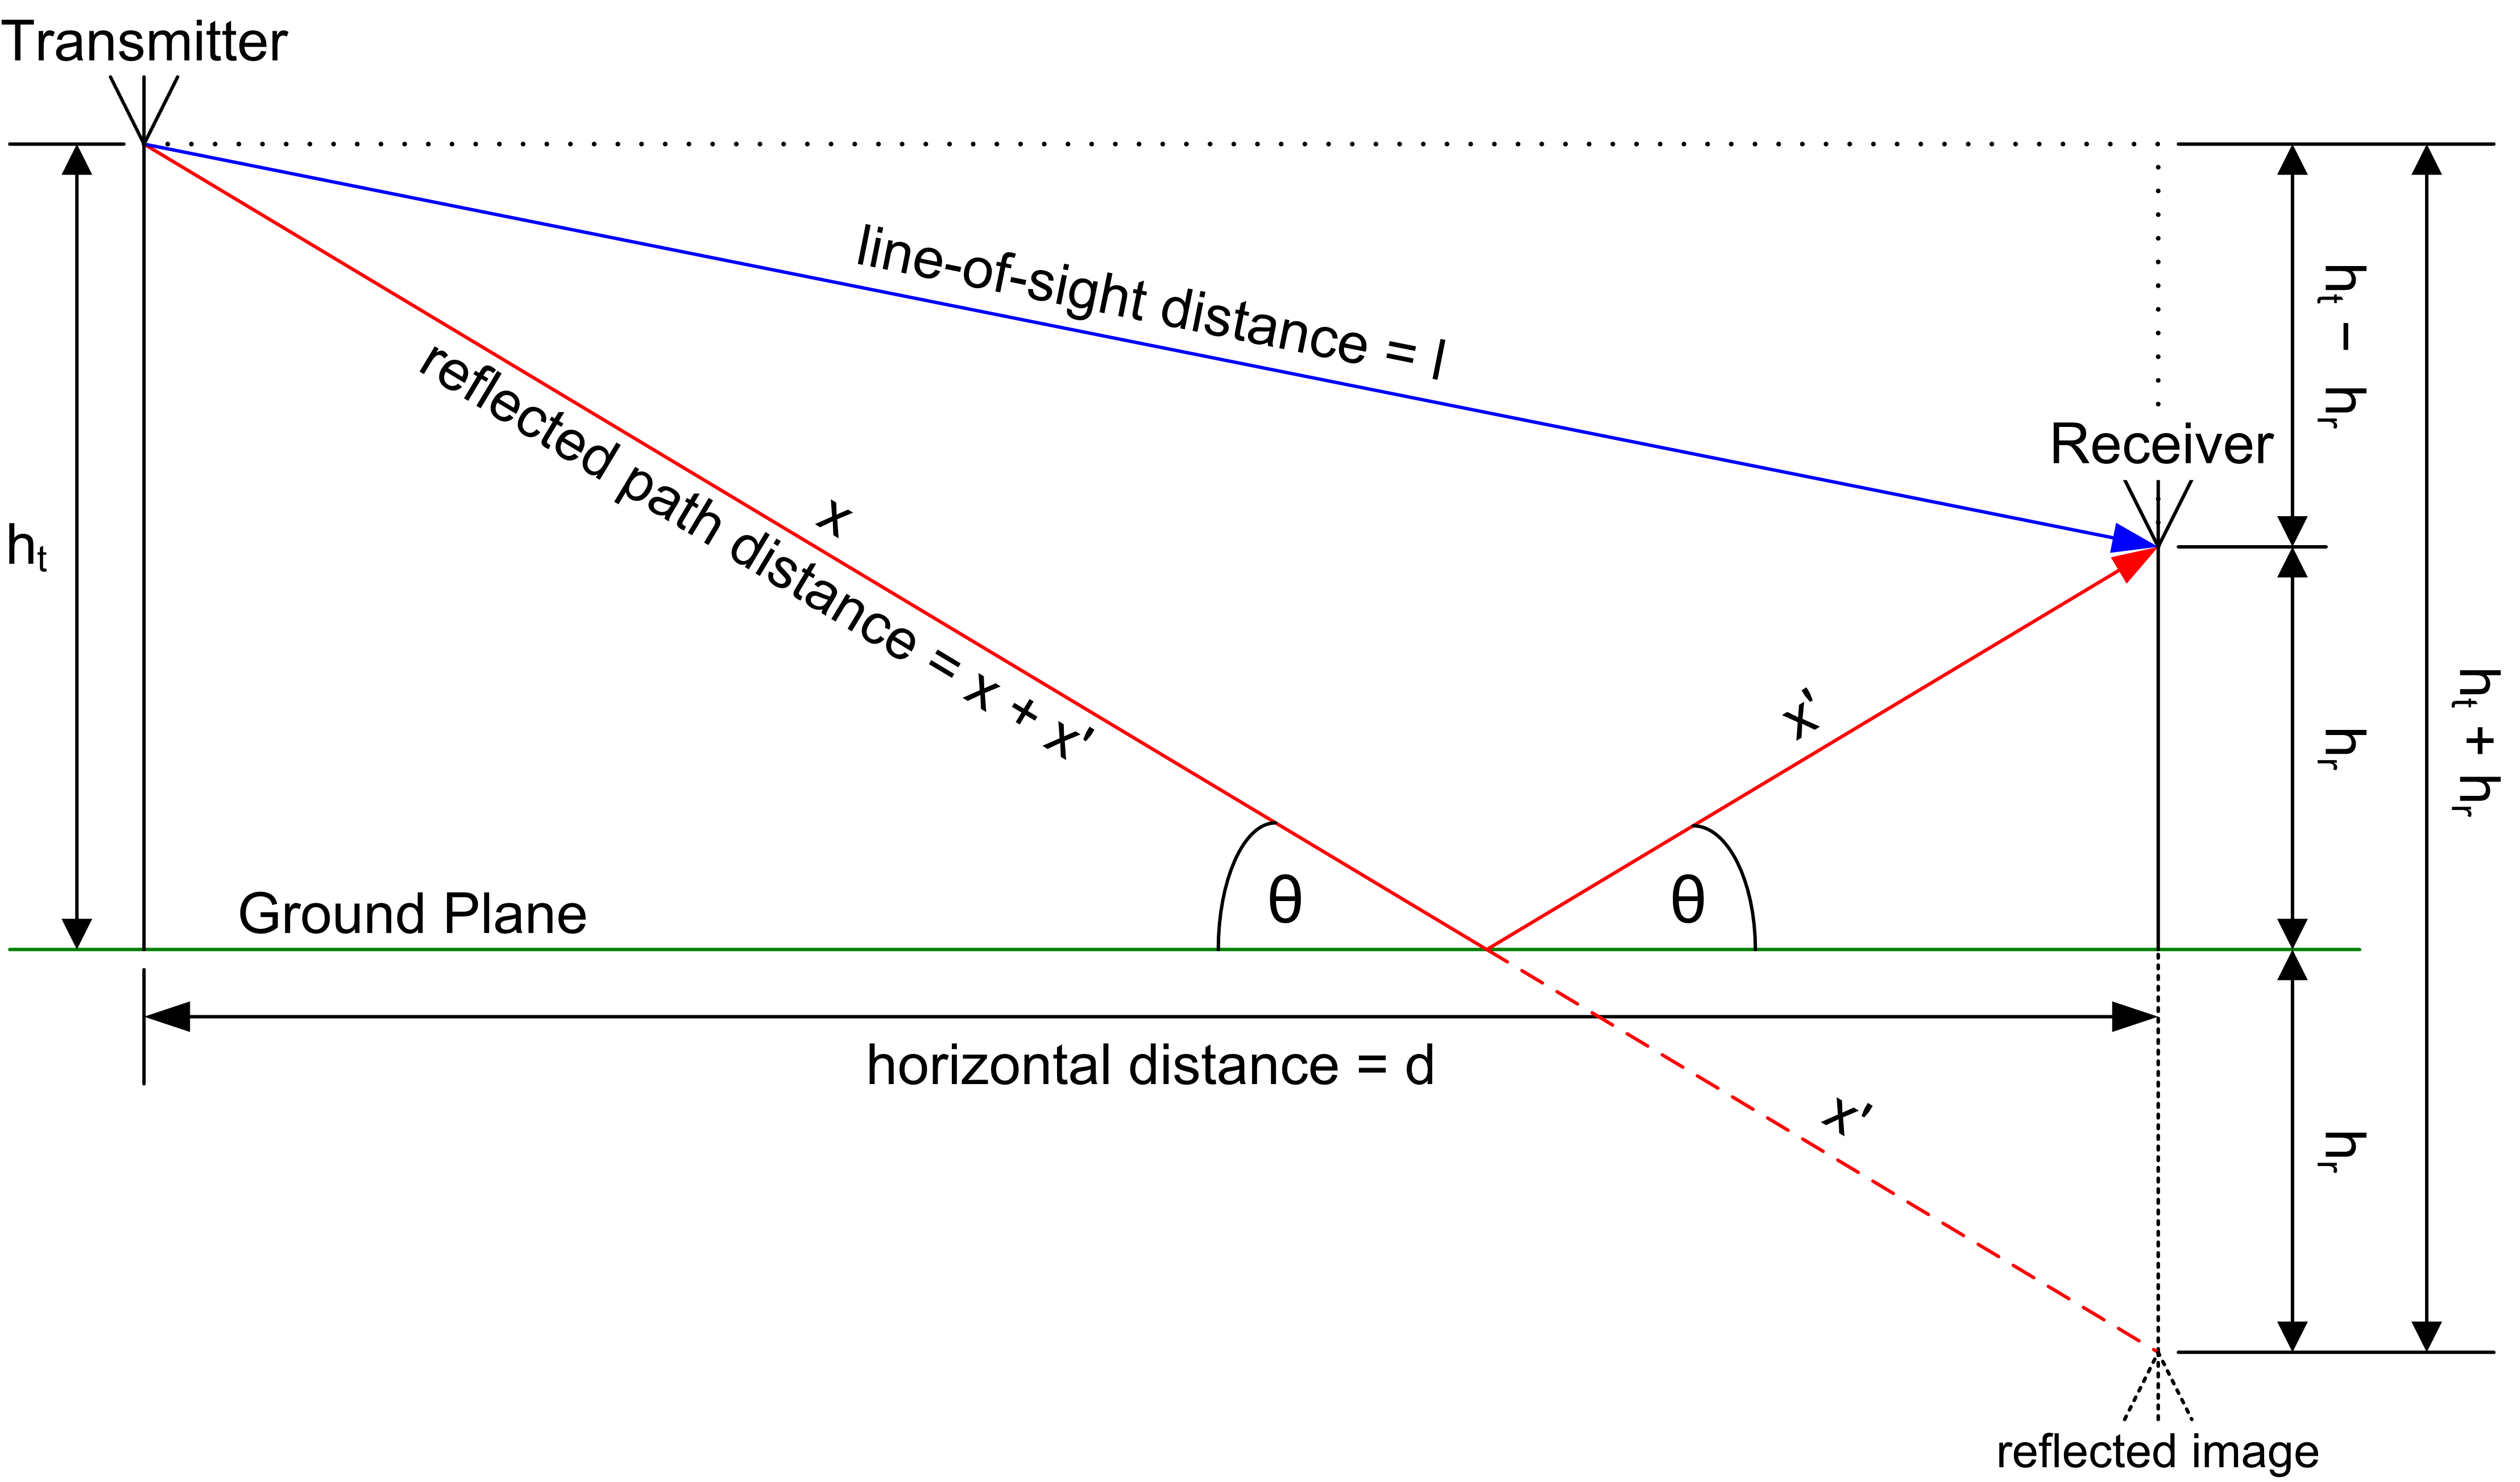
\includegraphics[scale=0.6]{2-Ray_Ground_Reflection.png}
		\caption{The paths travelled by the signal in the 2-ray ground propagation loss model }
	\end{figure}

	The receiver's power is given by the equation:
	
	\[P_r = \dfrac{P_t\cdot G_t \cdot G_r\cdot (h_t^2 \cdot h_r^2)}{d^4 \cdot L}\]
	
	Thus the power is proportional to $\frac{h_t^2 \cdot h_r^2}{d^4}$.
	
	At a short distance, superposition of the wavelength can be problematic, and so the Friis model is used instead. In our case, with the antenna height of 0.1 m, this crossover distance is roughly equal to 1.2 m. Thus it is not relevant to our simulations.
	
	\subsection{Question 2c.i}
	We start our simulations with a wavelength of 0.10 m, as before, which gives us frequency of $3 \times 10^9$ Hz. We begin with a distance of 180 m, however no packets are received at this range. 
	
	Even after increasing the transmission power to over 20 dBm (which is in accordance with the 802.11 standard). We suspect that the reason behind it is that for a small values of $\theta$, the direct and the reflected paths are very close together and running almost parallel, therefore causing a lot of interference.
	
	\subsection{Question 2c.ii}
	We take readings at a distance ranging from 15 to 15.09 m, in 0.01 m intervals. The results are summarised in the graph below.
	
	\begin{figure}[h]
		\centering
		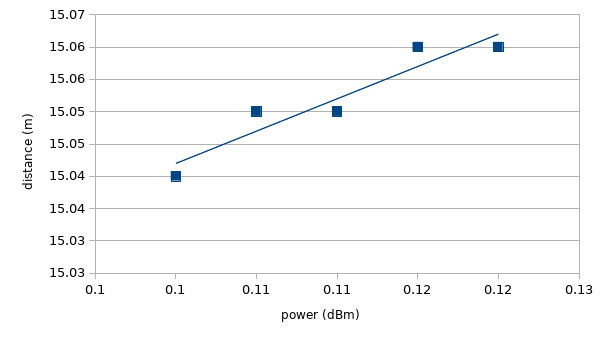
\includegraphics[scale=0.6]{graph_2ray1.png}
		\caption{Two ray ground reflection model, with antenna height of 0.1m}
	\end{figure}

	All packets below the recorded distance were received. This may be a little surprising, as the antenna length is the same as the wavelength. Despite trying with much smaller intervals of the distance, and antenna heights shorter than the wavelength, we consistently had all packets received up to a certain maximum distance.

	\subsection{Question 2c.iii}
	With a taller antenna, the signal easily reaches further. For example, with an antenna 0.15 m tall we found that the packets were received at all the above distances. In fact, the range in this case is around 22.5 m.
	
	\subsection{Question 2c.iv}
	The results of increasing the z coordinate of the nodes to 0.15m, while having antenna height of 0 m are the same as the range for an antenna height of 0.15 m. This is not surprising - according to the NS-3 specification, the values used for the vertical location of the nodes for calculations, are the z coordinate plus antenna height.
	
	\section{Conclusion}
	
	We have looked at four propagation loss models: one abstract one and three more realistic ones. The latter have various uses and are suitable for different scenarios. For example, log distance model is appropriate for simulating a suburban environment, while Friis model requires empty space. While that is unrealistic at long distances, it is suitable for calculating the loss at a very short distance, at which other models give impossible results.
	
	The maximum distance reached by each model is summarised in the table below.
	
	\begin{table}[h]
		\centering
		\begin{tabular}{|c|c|c|c|c|c|}
			\hline
			Model& TXp 0.1 dBm & TXp 0.105 dBm & TXp 0.11 dBm & TXp 0.115 dBm & TXp 0.12 dBm \\
			\hline
			Log-distance & 180.4 & 180.5 & 180.55 & 180.6 & 180.7 \\
			\hline
			Friis & 180 & 180.1 & 180.2 & 180.4 & 180.5 \\
			\hline 
			Two-ray ground & 15.04 & 15.05 & 15.05 & 15.06 & 15.06 \\
			\hline
			Range &180.5 &180.5 & 180.5 & 180.5 & 180.5\\
			\hline
		\end{tabular}
	\caption{Range achieved by the models for a given transmitting power (TXp), measured in metres.}
	\end{table}
	\pagebreak	
	
	\begin{thebibliography}{1}
		\bibitem{log distance doc}
		Log distance propagation loss model, NS-3 documentation, \url{https://www.nsnam.org/docs/release/3.19/doxygen/classns3_1_1_log_distance_propagation_loss_model.html}
		
		\bibitem{friis doc}
		Friis propagation loss model, NS-3 documentation
		\url{https://www.nsnam.org/docs/release/3.19/doxygen/classns3_1_1_friis_propagation_loss_model.html}
		
		\bibitem{friis note}
		H. Friis, "A note on simple transmission formula" in \emph{Proc. IRE}, May 1946, pp 254-256
		
		\bibitem{Shaw}
		J. Shaw, "Radiometry and the Friis transmission equation" in \emph{Am. J. Physics}, 2013, pp 33–37
		
		\bibitem{range doc}
		Range propagation loss model, NS-3 documentation, \url{https://www.nsnam.org/docs/release/3.19/doxygen/classns3_1_1_range_propagation_loss_model.html}
		
		\bibitem{two ray doc}
		Two-ray ground propagation loss model, NS-3 documentation, \url{https://www.nsnam.org/docs/release/3.19/doxygen/classns3_1_1_two_ray_ground_propagation_loss_model.html}
		
		\bibitem{NS3_comparison}
		M. Stoffers and G. Riley, "Comparing the ns–3 Propagation Models" in \emph{IEEE 20th Int. Symp. Modelling, Analysis and Simulation of Computer and Telecommunication Systems}, Aug. 2012, pp 61-67
		
	\end{thebibliography}
	
	
	%\IEEEPARstart{}{} 
	

	
	% that's all folks
\end{document}

